

\documentclass[10pt, conference, compsocconf]{IEEEtran}
\usepackage{graphicx}
\graphicspath{ {images/} }
\hyphenation{op-tical net-works semi-conduc-tor}


\begin{document}

\title{Collision Prevention in Distributed 6TiSCH Networks }




\author
{
		\makebox[.33\linewidth]{\fontfamily{ptm}\selectfont Ali J. Fahs}\\ \textit{DRAKKAR - Synchrone} \\\textit{LIG-VERIMAG}\\ \textit{Grenoble,France} \\\textit{ali.fahs@etu.univ-grenoble-alpes.fr}\\\
\and 	\makebox[.33\linewidth]{\fontfamily{ptm}\selectfont Olivier Alphand}\\ \textit{DRAKKAR Team} \\ \textit{LIG} \\\textit{Grenoble,France}\\\textit{olivier.alphand@imag.fr}\\\   
\and	\makebox[.33\linewidth]{\fontfamily{ptm}\selectfont Franck Rousseau}\\ \textit{DRAKKAR Team} \\ \textit{LIG}\\\textit{Grenoble,France}\\\textit{franck.rousseau@imag.fr}\\\   
\and 	\makebox[.33\linewidth]{\fontfamily{ptm}\selectfont Karine Altisen }\\ \textit{Synchrone}\\ \textit{VERIMAG}\\\textit{Grenoble,France}\\\textit{karine.altisen@imag.fr}\\\
\and 	\makebox[.33\linewidth]{\fontfamily{ptm}\selectfont St\'ephane Devismes}\\ \textit{Synchrone}\\ \textit{VERIMAG}\\ \textit{Grenoble,France} \\\textit{stephane.devismes@imag.fr}\\\
\and 	\makebox[.33\linewidth]{\fontfamily{ptm}\selectfont Rodolphe Bertolini}\\ \textit{DRAKKAR Team}\\ \textit{LIG}\\\textit{Grenoble,France}\\\textit{bertolir@etu.univ-grenoble-alpes.fr} \\\

}


\maketitle


\begin{abstract}
The abstract goes here. DO NOT USE SPECIAL CHARACTERS, SYMBOLS, OR MATH IN YOUR TITLE OR ABSTRACT.

\end{abstract}

\begin{IEEEkeywords}
 \hspace{.1cm} IoT ; WSN ; IEEE802.15.4e ; 6TiSCH ; 6top

\end{IEEEkeywords}




\IEEEpeerreviewmaketitle



\section{Introduction}

Network Technologies have been shifted from a limited number of interconnected expensive computers with high performance processing units to networks made of a huge number of  cheap entities with limited processing capabilities, called {\em things}, leading to the idea of {\em Internet of Things (IoT)}. The communication between those entities has required the creation of a standard, {\em IEEE802.15.4}.

IEEE802.15.4 aims at offering the low network layers ({\em i.e.}, PHY and MAC) for low cost and low speed communication. Actually, the contribution of this standard is not only limited to the reduction of the power consumption, but also to use techniques reducing  the manufacturing cost. All of this was managed while achieving network reliability. 

In 2012, {\em TSCH (Time-Slotted Channel Hopping)} was proposed by  {\em IETF (Internet Engineering Task Force)} and added to the media access layer of IEEE802.15.4e. TSCH is Time-slotted which means that there is periodic slot-frame. This slot-frame is split into several time-slots. The length of the time-slots should be large enough to send the maximum frame length from the transmitting node (Tx) to the receiving node (Rx), while ensuring synchronization between nodes. TSCH is also based on channel hopping, where the bandwidth is split over several channels. Consequently, many nodes can communicate at the same time-slot using different channels, identified by channel offsets. Two nodes willing to communicate have to pick up a cell from the TSCH table. This cell is defined by the number of time-slot (0 $\rightarrow L-1$, where $L$ is the slot-frame length) and a channel offset. There are two types of TSCH cells: the shared cells where each node is either listening, or sending; and the dedicated cells that provide private communication between two neighboring nodes. 

Since we are dealing with millions of nodes, sensors, and things that should be connected to the Internet, large scaling capabilities are mandatory. This was the focus of IETF Working Group, which has created the 6TiSCH architecture to enable IPv6 over TSCH in the existing IEEE802.15.4e.
\begin{figure}[h]
    \centering
    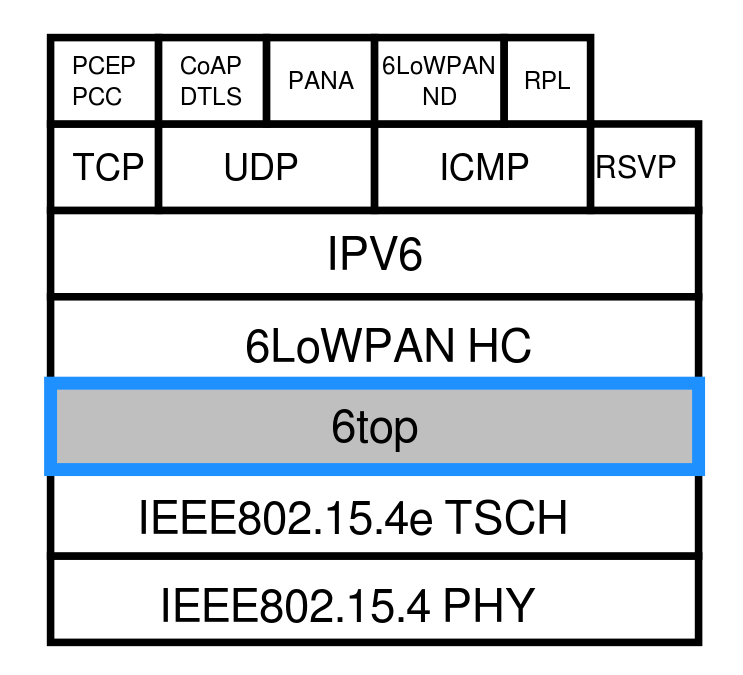
\includegraphics[width=4.77cm, height=4cm]{layers.png}
    \caption{Layers of the 6TiSCH Networks}
    \label{fig:Layers of the 6TiSCH Networks}
\end{figure}

In this paper we focus on the 6TiSCH operation sublayer (6top) that  allows neighboring nodes to add and/or delete TSCH dedicated cells. In addition, we are concerned about the scheduling function which selects cells to be assigned to nodes.

 The complexity of the problem lays on the fact that the system is distributed, {\em i.e.}, there is no central entity to monitor the whole network. Precisely, the resource allocation process (adding or removing cells) should be done locally, using the communication between the neighboring nodes in the shared cells. The communication is organized as a distributed convergecast to a sink node and based on a {\em Destination-Oriented Directed Acyclic Graph (DODAG)} computed by the  {\em Routing Protocol for Low-Power and Lossy Networks (RPL)}. Hence during a communication in the dedicated slot, Rx is necessarily a parent of Tx.  

The scheduling function in 6top selects cells from the TSCH schedule to be assigned to the pair of nodes asking for new communication cells. This process has to consider many fact
Since the scheduling function ignores the cells reserved by the neighbors, the network is subjected to collisions in dedicated cells, {\em i.e.}, two neighboring nodes that are not directly linked in the DODAG can select the same cell, leading to collisions, and consequently packet dropping. Our contribution focuses on reducing those collisions. For that reason, we take the cells used in the neighborhood into account during the cell allocation. Moreover we have to take the latency and the contention in the shared slot into account while implementing our approach.

The solution we have implemented achieves a minimum reduction of 66 \% in the number of collided Tx cells, and … \% reduction of the number collided packets. As a positive side-effect we observed a significant reduction of interferences in the network. \\

The main contributions of our papers are:

\begin{itemize}
\item Implementing a mechanism to collect the dedicated cells reserved by neighbors without introducing any overhead to the network. 
\item Modifications of the add and delete operations at the 6top sublayer, to force 6top to consider the neighboring nodes while reserving a new cell.
\end{itemize}

\section{Background}

\subsection{6TiSCH Operation Sublayer (6top)} 

IEEE802.15.4e has standardized TSCH medium access layer. However the mechanisms to build and manage the communication schedule were not defined in this standard, because the aim was to allow flexible customization and optimization. TSCH and IPv6 have been merged into 6TiSCH, whose operation sublayer, 6top, aims at managing the TSCH.

6p (6top protocol) which is a part of 6top, orchestrates all communications using the TSCH schedule. 6P controls the cell reservation and deletion process. It allows the nodes to request for new TSCH cells and update the TSCH schedule accordingly. Hence 6P enables the distributed scheduling in 6TiSCH network.

If we consider a Tx node (child) and Rx node(parent) that are communicating in the 6TiSCH network, 6P can achieve 3 types of operations for this communication: 
\begin{enumerate}

\item Tx determines that it need more cells to communicate with Rx. Then, it  will issue a 6top transaction to add more cells into TSCH schedule. Notice that one of  the duties of the scheduling function in 6top is to decide if more cells are needed.

\item Tx determines that it need less cells to communicate with Rx. Then, it will issue a 6top transaction to delete some TSCH cells. 

\item In some cases, Tx and/or Rx detect a dedicated cell facing collisions. As a result, Tx replace the defected cell through 6top transactions, this process is called {\em cell relocation}.
 
\end{enumerate}

Each operation is encapsulated into a transaction. A  6top transaction consists in a negotiation between Tx and Rx, that induce an update in the TSCH table. This transaction can consist of 2 or 3 steps. As shown in Figure 2, the 2 steps transaction start with the child (Tx) sending a request with available cells to be reserved, the parnet reply with the selected cells. Meanwhile the 3 steps transaction start with Tx sending a request for new cells, this request is followed by a reply from Rx with the available cells to be reserved, finally tx will reply with an acknowledgment that contain the reserved cells. 

In 6P transaction, the scheduling function decides to use 2 steps transaction, 3 steps transaction, or a mix between them. Also the scheduling function decides how to send the available cells, where we have two types to refer to them: 
\begin{enumerate}

\item Black listing: where the node sends all the cells it's already using.

\item White listing: where the node sends a number of nodes that are feasible for communication. 



\end{enumerate}


   

\begin{figure}[h]
    \centering
    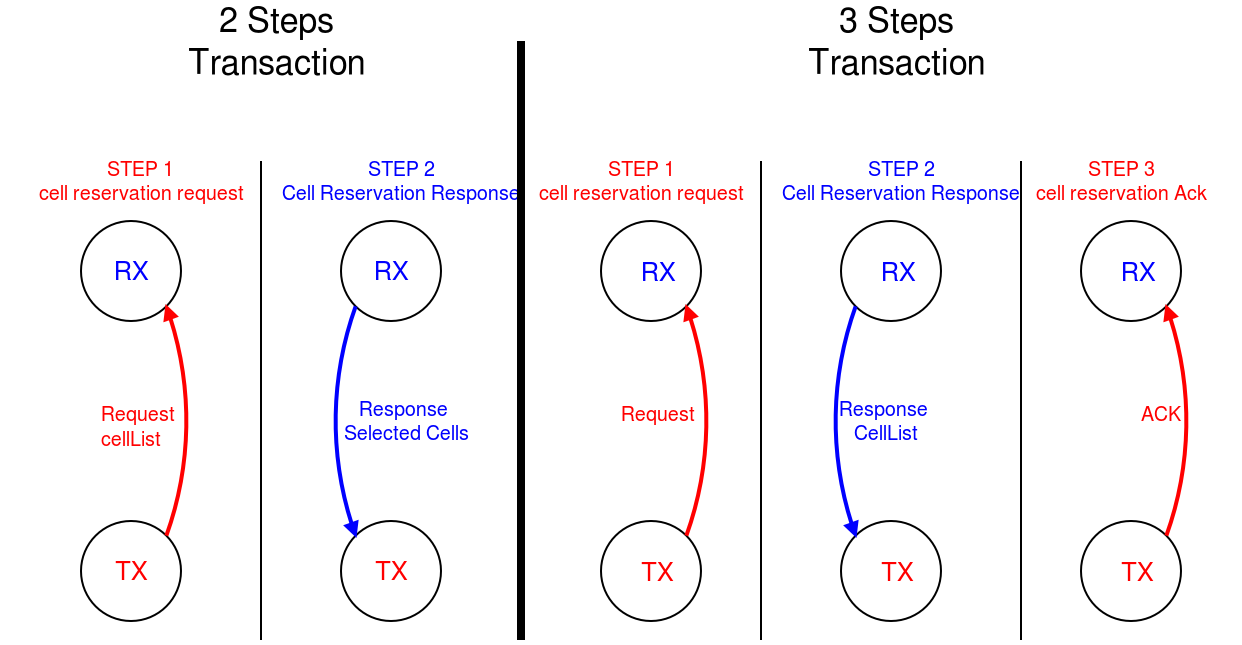
\includegraphics[width=9cm, height=4.5cm]{2,3steps.png}
    \caption{6P Transaction}
    \label{fig:Collision in 6TiSCH Networks}
\end{figure}



The scheduling function determines which transaction to be used. Transactions are done in the shared slot, which means that they can be received by the neighboring nodes. However, due to the filtering at the MAC layer, those transactions are actually ignored .


\subsection{Medium Access Control Filtering}

Consequently, According to the IEE802.15.4 which defines the MAC layer, the filtering is done over levels of filters, such that the first level  will filter out the defected messages using FCS (frame check sequence),the second and the third filters will check specific modes in the network and act correspondingly , the final level of  filtering deals with the content of the frame. Out of our scope we are mostly interested in the final MAC filtering layer , where the MAC layer decides whether to pass the frame to the next level or not, according to list of conditions like {\em frame type, version and detestation PAN ID}.

We can manipulate those conditions by two ways, either by sending a frame that we confirm it will pass those conditions, or by changing the setting in the MAC layer  by adding new conditions. As an example we can add a condition in the MAC layer to accept all the frame with the frame version \verb|IANA_6TOP_6P_VERSION|. Frames with this version are the frames transmitted by 6top protocol according to the IETF standards for 6top.

Further in explanations, we can use the fact that the 6p transaction are submitted in the shared slot. Also we can modify the MAC filtering in a way that allows neighbors to collect the informations contained in the 6P transaction. This information can divert neighboring nodes from selecting cells already in use, consequently reducing notably the collisions.

\subsection{Collisions in the Dedicated Cells }

The probability of collision is direclty related to the number of nodes, and more precisely to the traffic of the network, {\em i.e.,} the more the network is congested, the more collisions will occur. In wireless sensor networks collisions are expensive in the means of power consumption and  end-to-end latency. As a result collisions in the dedicated cells of TSCH should be reduced, and for that purose it should be investigated more. 


 Collisions occur at the reception node, where the neighboring nodes of Rx are the only nodes that can induce collision. That will take place if Rx have two or more neighbors transmitting using the same scheduled cell, one of these nodes must be a child, the reset are neighbors transmitting to their parents. 
   
Collisions in in dedicated cells is the core of the problem we are trying to solve. 
\begin{figure}[h]
    \centering
    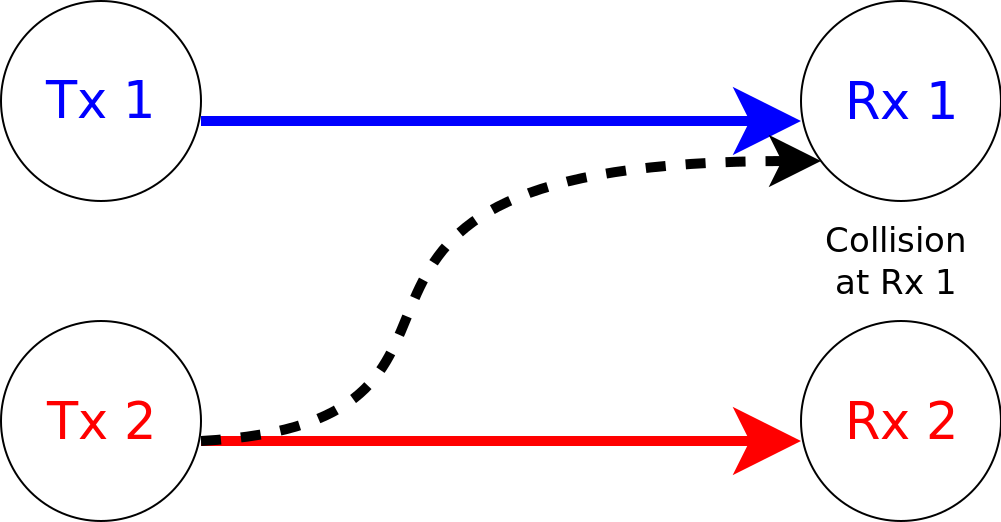
\includegraphics[width=6.5cm, height=3.2cm]{collision.png}
    \caption{Collision in 6TiSCH Networks}
    \label{fig:Collision in 6TiSCH Networks}
\end{figure}



\section{Proposed Mechanism}

In the previous section we have defined IEEE802.15.4e TSCH schedule, and the problem occurring in the dedicated cells of this schedule. The main reason of this problem is the distributed mechanism used to select communication cells, where if we had a central entity assigning cells to the nodes, the problem will not exist. 

Our solution is built based on the idea of mutual exclusion. When a pair of Rx and Tx nodes reserve a new communication cell, Rx must inform it's neighbors which cell or set of cells are reserved. 

The main idea was to use broadcast in the shared cell to inform the neighbors each time a cell is reserved, but the shared cell is already congested, and broadcasting each time a cell is reserved is an overhead to the network. The overhead induced by such approach is much more expensive than the collision reduced. 

The twist in our approach is the use of the already existing 6P transactions. the 6P transaction are submitted in the shared slot and received by the neighbors in the PHY layer, they are then dropped due too the MAC filtering. If we apply a slight modification at the MAC sublayer we can prevent filtering those transaction, and consequently, collecting the cells reserved by the neighbors. This was achieved without introducing any new overhead to the network. 

In case the scheduling function uses 2 steps transactions we can collect the cells reserved by Rx from the reply, using white listing. However if the scheduling function uses the 3 steps transaction, we can collect the cells of Rx using black listing when Rx reply. By this we can assure that we are able to keep track of the neighbor's cells so we can avoid collision. 
\subsection{The Avoid Table}

After collecting the cells they will be saved in a table, we call it the {\em avoid table}. The structure of this table is similar to that of TSCH, where each cell is represented by a time-slot and a channel offset and refer to the cell with the same coordinates in TSCH. the cell in Avoid can be marked as available of reserved, where available means it can be used for communication since no neighbors are using this cell, and if it's marked as reserved, then it should be avoided for the possibility of collision.

In Figure 4. we can see the structure of the avoid table.****


 
\begin{figure}[h]
    \centering
    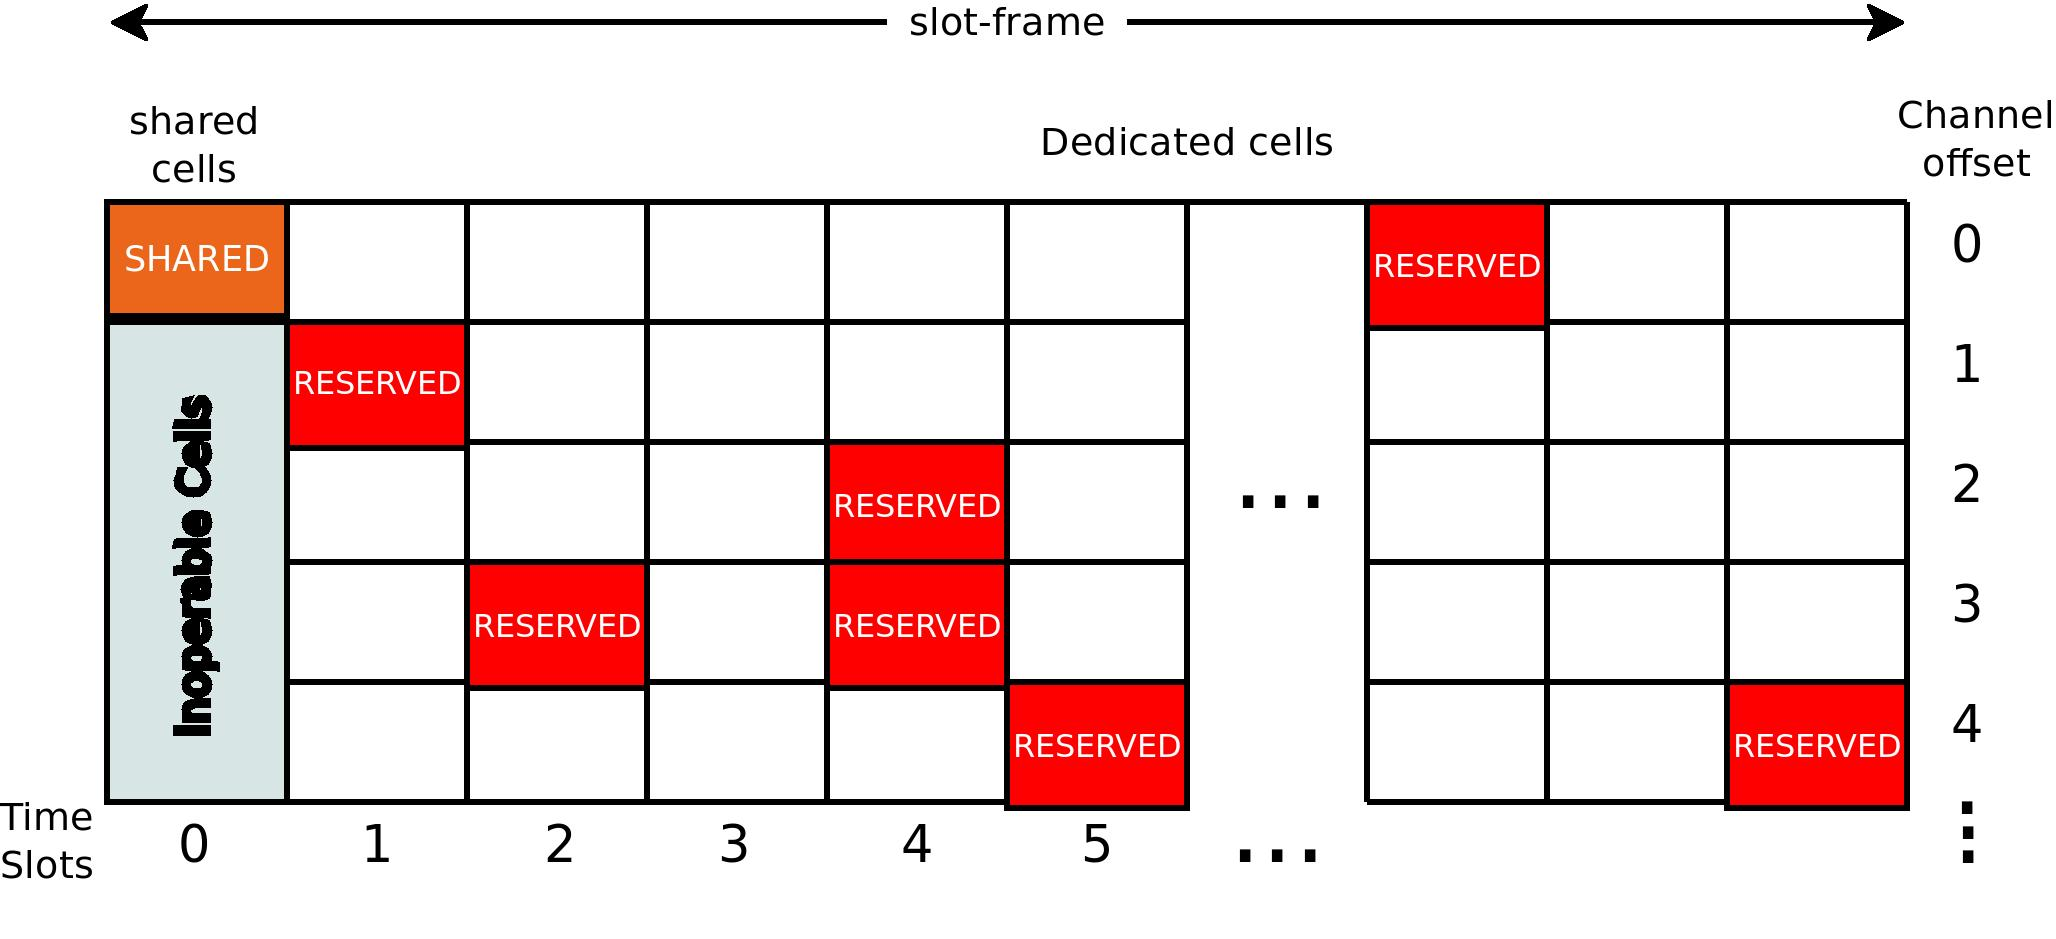
\includegraphics[width=8cm, height=4cm]{avoid.jpeg}
    \caption{The Avoid table}
    \label{fig:Collision in 6TiSCH Networks}
\end{figure}

The last step of this mechanism lays on forcing the scheduling functions to follow the avoid table, one of our goals in this implementation is the flexibility of the mechanism with different  scheduling functions, as a result our implementation is supposed to be in the 6top sublayer. 6top have to force the scheduling function to avoid the cells found in the avoid table. using this mechanism can assure us a collision free dedicated cell if we have 100\% successful transmission of the 6P transaction to all neighbor nodes, which is obviously unrealistic.

The 6p transaction is submitted from the Rx node to the Tx node in wireless medium, for this transaction to reach all the neighbors we should have a perfect conditions in the network which is something we don't have especially in wireless sensor networks. As a result of environment factors the 6P transaction is delivered to a part of the neighborhood where for some node the transaction will be lost. This fact will again induce collision for the same reasons explained previously, yet by using such an approach we will still get a reduction in the probability of collisions, but not as we want.**** 

\subsection{Cell buffer}

To reduce the effect of the lost 6P transactions in the probability of collisions, we added a cell a buffer that store the last $k$ cells reserved by node with it's children. The length of this buffer is $k$.  Whenever a cell is reserved, instead of sending only the reserved cells, the cell buffer will be sent also, as a result all the cells in the buffer will be added to the avoid table. Technically, that means that each cell will be transmitted $k$ times to the neighborhood instead of once, as in the  approach. That have effectively increased the probability of successful reception of 6P transaction and consequently reduce the probability of collisions. 

     


 	
\section{Results}

\section{Related Work}

\section{Conclusion}



\section*{Acknowledgment}
The authors would like to thank...
more thanks here




\begin{thebibliography}{1}

\bibitem{IEEEhowto:kopka}
Q.Wang, and X. Vilajosana, \emph{ 6top Protocol (6P). Internet Engineering Task Force, Tech. Rep. draft-ietf-6tisch-6top-protocol-00 } \hskip 1em plus
0.5em minus 0.4em\relax https://tools.ietf.org/html/draft-ietf-6tisch-6top-protocol-00 , April 2016.

\bibitem{IEEEhowto:kopka}
T. Watteyne et al, \emph{ Using IEEE 802.15.4e Time-Slotted Channel Hopping (TSCH) in the Internet of Things (IoT): Problem Statement } \hskip 1em plus
  0.5em minus 0.4em\relax https://tools.ietf.org/html/rfc7554 , May 2015.

\bibitem{IEEEhowto:kopka}
T. Winter et al, \emph{ RPL: IPv6 Routing Protocol for Low-Power and Lossy Networks } \hskip 1em plus
  0.5em minus 0.4em\relax https://tools.ietf.org/html/rfc6550 , March 2012.

\bibitem{IEEEhowto:kopka}
D. Dujovne et al, \emph{6tisch: deterministic ip-enabled industrial internet(of things)} \hskip 1em plus
  0.5em minus 0.4em\relax IEEE Communications Magazine — Communications Standards Supplement ,December 2014.
  
\bibitem{IEEEhowto:kopka}
J. Tripathi et al, \emph{A Performance Evaluation Study of RPL: Routing Protocol for Low Power and Lossy Networks} \hskip 1em plus
  0.5em minus 0.4em\relax  Information Sciences and Systems (CISS), 44th Annual Conference on (pp. 1-6). IEEE , March 2010.

\bibitem{IEEEhowto:kopka}
F. Theoleyre and G. Papadopoulos, \emph{Experimental Validation of a Distributed Self-Configured 6TiSCH with Traffic Isolation in Low Power Lossy Networks} \hskip 1em plus
  0.5em minus 0.4em\relax  Proceedings of the 19th ACM International Conference on Modeling, Analysis and Simulation of Wireless and Mobile Systems (pp. 102-110). ACM , November 2017.
  
\bibitem{IEEEhowto:kopka}
N. Accettura et al, \emph{A Decentralized Traffic Aware Scheduling in 6TiSCH Networks: Design and Experimental Evaluation} \hskip 1em plus
  0.5em minus 0.4em\relax   IEEE Internet of Things Journal, 2(6), 455-470 , December 2015.
  
\bibitem{IEEEhowto:kopka}
M. R. Palattella et al, \emph{On-the-Fly Bandwidth Reservation for 6TiSCH Wireless Industrial Networks} \hskip 1em plus
  0.5em minus 0.4em\relax  IEEE Sensors Journal, 16(2), 550-560,  September 2015.
  
\bibitem{IEEEhowto:kopka}
M. R. Palattella et al, \emph{Traffic Aware Scheduling Algorithm for Reliable Low-Power Multi-Hop IEEE 802.15.4e Networks} \hskip 1em plus
  0.5em minus 0.4em\relax  IEEE 23rd International Symposium on Personal, Indoor and Mobile Radio Communications - (PIMRC),  September 2012.
 
\bibitem{IEEEhowto:kopka}
N. Accettura et al, \emph{Decentralized Traffic Aware Scheduling for Multi-hop Low Power Lossy Networks in the Internet of Things} \hskip 1em plus
  0.5em minus 0.4em\relax   In World of Wireless, Mobile and Multimedia Networks (WoWMoM), 2013 IEEE 14th International Symposium and Workshops on a (pp. 1-6). IEEE,  June 2013.
 
\bibitem{IEEEhowto:kopka}
S. Duquennoy et al, \emph{Orchestra: Robust Mesh Networks Through Autonomously Scheduled TSCH} \hskip 1em plus
  0.5em minus 0.4em\relax  Proceedings of the 13th ACM Conference on Embedded Networked Sensor Systems (pp. 337-350). ACM, November 2015.

\bibitem{IEEEhowto:kopka}
K. Muraoka et al, \emph{Simple Distributed Scheduling With Collision Detection in TSCH Networks} \hskip 1em plus
  0.5em minus 0.4em\relax  IEEE Sensors Journal, 16(15), 5848-5849,  May 2016.
  
\bibitem{IEEEhowto:kopka}
L. Lamport, \emph{Time, clocks, and the ordering of events in a distributed system} \hskip 1em plus
  0.5em minus 0.4em\relax  Communications of the ACM, 21(7), 558-565, July 1978.
  
\bibitem{IEEEhowto:kopka}
T. P. Duy , \emph{Distributed cell selection for scheduling function in 6TiSCH networks} \hskip 1em plus
0.5em minus 0.4em\relax Computer Standards and Interfaces, 53, 80-88, March 2017.

\end{thebibliography}

\medskip





\end{document}


